
%\graphicspath{{../figures/}{./gfx/}{/media/data/Work/cnstellate/golgi/}{../../cnstellate/}}

%===================================
\section[GLG Cell Model]{Golgi Cell Model: Optimisation using monotonic rate-level responses in marginal shell units \label{sec:GolgiCellModel}}

\subsection{Background}

The presence of GABAergic inputs to \VCN~and \DCN~neurons has been verified by labeled terminals adjacent to the soma and dendrites \citep{SmithRhode:1989,AwatramaniTurecekEtAl:2005,BabalianRyugoEtAl:2003} and release from inhibition in their response areas with ionotopopheretic application of the \GABAa~antagonist, bicuculine \citep{EvansZhao:1998,CasparyBackoffEtAl:1994,BackoffShadduckEtAl:1999,FerragamoGoldingEtAl:1998a}.
The source of GABAergic inputs to cells in the mammalian \CN~is somewhat contentious.
Studies show that GABAergic inputs to the \CN~generally arise in the peri-olivary regions of the medulla in cats \citep{OstapoffBensonEtAl:1997} and birds \citep{LachicaRubsamenEtAl:1995,YangMonsivaisEtAl:1999}.
Slice preparations of the isolated murine \VCN~show strong and immediate sensitivity to bicuculine in T~and D~stellate cells from a source within the \CN~complex \citep{FerragamoGoldingEtAl:1998a}.
The only known source of \GABA~intrinsic to the \VCN~are the Golgi cells of the \GCD~overlying the \VCN~\citep{Mugnaini:1985,FerragamoGoldingEtAl:1998}.

%\smallskip{}

% \yellownote{TODO: Clean up paragraph} Other studies in the rat cochlear
% nucleus relating to the Golgi cell or \GABA:
% \begin{itemize}
% \item \citep{MugnainiOsenEtAl:1980} Fine structure of granule cells and
%   related inter-neurons (termed {Golgi} cells) in the cochlear nuclear complex
%   of cat, rat and mouse
% \item \GABAa expression in the rat brainstem \citep{CamposCaboEtAl:2001}
% \item \citep{Alibardi:2003a} Ultrastructural distribution of glycinergic and
%   {{GABAergic}} neurons and axon terminals in the rat dorsal cochlear nucleus,
%   with emphasis on granule cell areas
% \item \citep{AwatramaniTurecekEtAl:2005} Staggered {Development} of
%   {GABAergic} and {Glycinergic} {Transmission} in the {MNTB}
% \end{itemize}

% %\smallskip{}

% \yellownote{TODO: Expand role of \GABA, or combine with previous para} Role of
% \GABA in the \VCN\@.
% \begin{itemize}
% \item Effects of microiontophoretically applied glycine and {GABA} on neuronal
%   response patterns in the cochlear nuclei \citep{CasparyHaveyEtAl:1979}
% \end{itemize}
% \citep{Alibardi:2003a} rat \CN~complex -> Golgi-stellate cells (fusiform layer:
% 2) in \DCN~contact granule and unipolar brush cells

Inputs to Golgi cells are more complicated than the inputs to core \VCN~neurons.
Golgi cells are sparse in the \GCD, surrounded by the many, smaller excitatory granule cells, that form small en-passant endings.
Type II \ANFs~create diffuse glutamatergic release sites in the \GCD~\citep{HurdHutsonEtAl:1999,BensonBrown:2004} that may stimulate NMDA glutamate receptors in Golgi cells~\citep{FerragamoGoldingEtAl:1998a}.

%\smallskip{}

The physiological response of Golgi cells has not been extensively studied.
Intracellular recordings of Golgi cells in one study by \citet{FerragamoGoldingEtAl:1998} have shown a classic type I current response.
This suggests Golgi cells are simple integrators.
Their response to auditory nerve shocks were delayed by approximately 0.7~ms relative to the core \VCN~units \citep{FerragamoGoldingEtAl:1998}.
Extracellular recordings from labelled Golgi cells is not available in the literature; however, the \GCD~(or marginal shell of the \VCN~in cats) has been studied by one group \citet{GhoshalKim:1997} without direct labelling of recorded units.
Any extracellular spikes recorded in the \GCD~are most likely from Golgi cells since granule cell somata are less than $10 \mu{m}$ and their narrow axons are unlikely to elicit electrical activity in the electrodes.
The majority of recorded units showed a monotonic increase in firing rate with increasing sound intensity \citep[Figure~\ref{fig:GolgiKimFig2}][]{GhoshalKim:1997}.


Their monotonic responses to tones and noise over a wide dynamic range provides regulation of activity in granule cells.
The contribution of a delayed, negative feedback onto \VCN~units is analogous to automatic gain control provides strong evidence for regulation of activity in granule cells. The general assumption of the functional role of Golgi cells is to regulate granule cells but they may also provide automatic gain control to the principal VCN~units, primarily D and T stellate cells \citep{FerragamoGoldingEtAl:1998a}.

%\smallskip{}

\begin{figure}[htp!]
   \centering
  % \resizebox{3.5in}{!}{\includegraphics{NoFigure}}
  \resizebox{0.95\textwidth}{!}{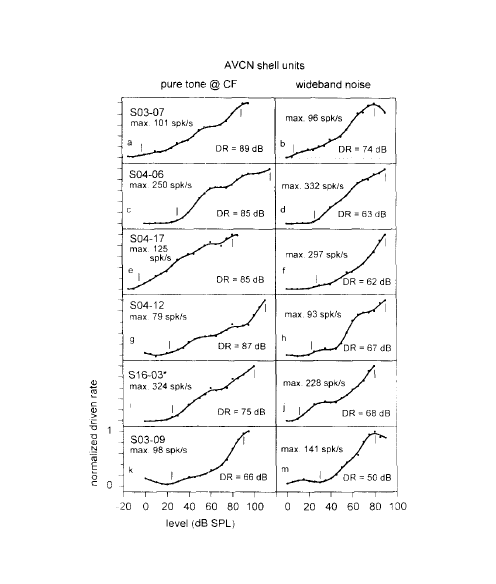
\includegraphics{GhoshalKim}}
  \caption[Rate level response of marginal shell units]{Rate level response of 6 units \citep[Reproduced with permission Fig.~2]{GhoshalKim:1997}.
Unit S03-07 (CF 22.7~kHz) at the top will be the unit chosen to optimise the Golgi cell model as it is monotonic, and has the median maximum rate of all the units shown. \yellownote{Inclusion of Ghoshal figure needs permission, fill in caption}
\label{fig:GolgiKimFig2}}
\end{figure}

%===================================
\subsection{Implementation}

In the creation of the Golgi cell model, we can reduce the explicit behaviour of Golgi cells down to three major details:
 \begin{enumerate}
 \item Golgi cells are classic repetitively-firing neurons due to their type I~current clamp response \citep{FerragamoGoldingEtAl:1998},
 \item Golgi cells have a low maximum rate and large dynamic range to tone and noise increases, given marginal shell extracellular recordings of \citet{GhoshalKim:1997} could not come from granule cells, and
 \item The low threshold in Golgi cells, \citet{GhoshalKim:1997}, can\-not be due to \LSR~auditory nerve fibres.
The lack of extensive experimental data regarding type II \ANF~units, that do project to the \GCD, and granule cell response to acoustic input meant that a Poisson rate neural model would be preferred over the Hodgkin-Huxley type neural model.
Although \HSR~\ANF~terminals do not generally project into the \GCD, they are included in this model to provide some low level sound-induced activity.
 \item the minimum \EPSP~to shock of the AN~\citep{FerragamoGoldingEtAl:1998} and mean first spike latency to acoustic stimuli~\citep{GhoshalKim:1997} are significantly different from the core \VCN~units.
% by $\mu(f=CF)$ and $\sigma$ variables, which control
 \end{enumerate}

%\smallskip{}


The Golgi cell model is implemented as an instantaneous-rate Poisson rate model, shown in Table~\ref{tab:GolgiCellModelSummary}D and in Figure~\ref{fig:GolgiDiagram}.
The primary inputs are from the auditory model's instantaneous rate outputs with connections across frequency channels.
\HSR~and \LSR~\ANF~inputs to Golgi cells were determined the Gaussian distribution in units of channel separation in the network.
The weighted sum of \HSR~and \LSR~instantaneous-rate vectors are smoothed out by an alpha function mimicking a synaptic and dendritic smoothing filter.

%\smallskip{}

Table~\ref{tab:GolgiCellModelSummary}A shows the model summary for optimising the Golgi cell model.
As explained in the introduction, the Nordlie tables are used to communicate detailed neural models and networks for further replication by the computational neuroscience community.
The topology of the ventral cochlear nucleus follows the same tonotopic organisation of the auditory nerve, with 100 evenly spaced frequency channels.
The population of \ANFs~in Table~\ref{tab:GolgiCellModelSummary}B are zero because there is no need for spiking \ANF~neurons, only the instantaneous profiles of each frequency channel is used in the Golgi model.
The connectivity between \ANFs~and Golgi cells (Table~\ref{tab:GolgiCellModelSummary}C) is a simple place-based Gaussian spread, as explained in the introduction ($\S$~\ref{sec:CN:tonot-conn})

% {%
\small\linespread{0.5}
\noindent%
\begin{table}[!thb]
    \caption{Golgi cell model summary (Nordlie format)}
    \label{tab:GolgiCellModelSummary}
\begin{tabularx}{\textwidth}{|l|X|} %
\hdr{2}{A}{Model Summary}\\
%\begin{ntab}{|l|X|}{2}{\ref{tab:GolgiCellModelSummary} A}{Model Summary}\\\hline
 \textbf{Populations}  & ANF~(HSR, LSR) and Golgi (GLG) cells \\\hline 
  \textbf{Topology}    & Tonotopic - 100 frequency channels (0.2--40
  kHz);  Cat model; Greenwood function centre frequencies \citep{Greenwood:1990}\\\hline
\textbf{Connectivity}  & ANF to GLG filter inputs, Gaussian spread
centred on channel\\\hline
\textbf{Input model}  & ANF~model: Version 4 and 5 Zilany model \citep{ZilanyBruce:2007,ZilanyBruceEtAl:2009} \\\hline
\textbf{Neuron model}  & GLG cell model: Instantaneous-rate Poisson
neuron model \\\hline
\textbf{Synapse model} & Synapto-dendritic smoothing filter (alpha function) \\\hline
%    \textbf{Input}     & Pure tones (22.7 kHz, 50 ms, 5 ms on/off ramp, 20 ms delay), intensity range 0--100 dB~SPL   \\\hline
%\textbf{Measurements}  & Mean firing rate of Golgi cell instantaneous rate profile or PSTH sampled from Poisson spike-generator (25 repetitions) \\\hline
\end{tabularx}
\vspace{1ex}
%\end{ntab}

% - B ------------------------------------------------------------------------
\noindent%
\begin{tabularx}{\textwidth}{|l|X|X|}%
\hdr{3}{B}{Populations}\\
\textbf{Name} &                         \textbf{Elements}                          & \textbf{Number} \\\hline
     HSR      & Auditory nerve fibre model
     \citep{ZilanyBruce:2007,ZilanyBruceEtAl:2009} & Rate models only,
     1 per channel\\\hline
     LSR      & Auditory nerve fibre
     \citep{ZilanyBruce:2007,ZilanyBruceEtAl:2009} & Rate models only,
     1 per channel \\\hline
     GLG      &                 Instantaneous-rate Poisson neuron model                  & 1 unit (CF 22.7 kHz, channel 76)  \\\hline
\end{tabularx}
\vspace{1ex}

% - C ------------------------------------------------------------------------------
\noindent
\begin{tabularx}{\textwidth}{|l|l|l|X|}%
\hdr{4}{C}{Connectivity}    \\
     \textbf{Name}       & \textbf{Source} & \textbf{Target} & \textbf{Pattern} \\\hline
\multirow{2}{*}{\ANFGLG} &     {\HSR}      &      GLG      & 
Gaussian spatial convergence, centred on CF, spread parameter
(\sHSRGLG = 2). Weight (\wHSRGLG) to be optimised. \\
   &     {\LSR}      &      GLG      & 
Gaussian spatial convergence, centered on \CF.  Spread (\sLSRGLG) and weight (\wLSRGLG) to be optimised. \\\hline
\end{tabularx}
\vspace{1ex}
% - D ------------------------------------------------------------------------------
\noindent%
\begin{tabularx}{\linewidth}{|p{0.22\linewidth}|X|}
\hdr{2}{D}{Neuron and Synapse Model}\\
 \textbf{Name} & Golgi cell model \\\hline
 \textbf{Type} & Instantaneous-rate Poisson neural  model \\\hline 
%\raisebox{-4.5ex}{\parbox{\linewidth}{\textbf{Model Dynamics}}} & 
 \textbf{Model Dynamics} & %
% {\rule{1em}{0em}\vspace*{-1.5ex}\scriptsize%
% \begin{equation*}%
%  \begin{array}{r@{\;=\;}ll}
%   \mathbf{w}_{L,H}&  w_{LSR,HSR \to GLG}\,\mathcal{N}(i_{{\rm CF}},\sigma)    & \text{Gaussian weight mean at CF, \sigma^2=\sLSRGLG} \\ 
%   \alpha(t)      &\left( t  \exp(\frac{-t}{\Gtau}) \right)   &  \text{Synapto-dendritic filter with unit area} \\
%   g(t)           & \mathbf{w}_{L}\bullet\mathbf{L}+\mathbf{w}_{H}\bullet\mathbf{H} & \text{Sum of dot products} \\ % between weights and ANF rate matrices}\\ 
% %\mathbf{H},\mathbf{L} \to f(\text{channel},t) & \mathbf{w}_{H,L} \to f(\text{channel})\\
%              %      r(\mathbf{x})              &               \max\{\mathbf{x}(t-\dANFGLG) - x(0) + \Gspon,0\}                & \\
%  G(t)  &   \lfloor \, \alpha(t)\,\ast\,g(t) \,\rfloor                  & \text{Convolution of $\alpha(t)$ and $g(t)$ and rectification}\\
% % & \text{if } G(t) < 0 \,G(t)=0 & \text{rectification of Golgi model rate} \\
% \end{array} \end{equation*}\vspace*{-1.5ex}\rule{1em}{0em}}  \\\hline
%{\rule{1em}{0em}\vspace*{-1.5ex}%\scriptsize%
See Figure~\ref{fig:GolgiDiagram} and the GLG rate filter model
Equations~\ref{eq:GolgiWeights}--\ref{eq:GolgiConvolution}.
% ($g_{i}(t)$) used for
% the Golgi cell model. It was created using convolution of weighted ANF input rates
% and synapto-dendritic kernel ($\alpha_{\small\rm GLG}(t)$) with rectification. 
% \begin{equation*}%
%  \begin{array}{r@{\;=\;}l}
%  {\rm GLG}_{i}(t)  &  \alpha_{\rm GLG}(t)\,\ast\,g(t) \,\rfloor + \text{SR}_{\rm GLG} \quad \text{where} \\
%   \alpha(t)      &\left( t  \exp(\frac{-t}{\Gtau}) \right)   \quad  \text{and} \\
%   g(t)           & \mathbf{w}_{L}\bullet\mathbf{L}+\mathbf{w}_{H}\bullet\mathbf{H} 
% \end{array} \end{equation*}\vspace*{-1.5ex}\rule{1em}{0em}
%Preliminary rate, $g(t)$, is the sum of dot products between weight vectors and ANF rate matrices.
% Gaussian weight vectors have mean at CF and $\sigma^2=\sLSRGLG$.}  
\\\hline
 \textbf{Spiking} & Renewal Poisson process given instantaneous rate, ${\rm GLG}_{i}(t)$,  with refractory effects  \citep{ZilanyBruce:2007,Jackson:2003} \\\hline
\end{tabularx}
\vspace{2ex} 

% $\dag$\footnotesize{Synaptic filter, $\alpha(t)$, is normalised, by setting the
%   area under the alpha function to one. For a large enough filter length, the
%   alpha function integral ($\int \alpha(t) dt = (-\Gtau^2 - t \cdot \Gtau)\cdot
%   \exp(-\frac{t}{\Gtau})$) approximately equals $\Gtau^2$. In this case $10
%   \times \Gtau$ is used for the filter length.}  

% - E -----------------------------------------------------------------------------
\noindent
\begin{tabularx}{\linewidth}{|l|X|} %
\hdr{2}{E}{Optimisation}\\
\textbf{Input Stimulus} & Rate Level function, 22.7~kHz tone at SPL -15 to 90 dB (50 ms duration, 2 ms cosine squared on\slash off ramp, 20 ms delay)\\\hline 
\textbf{Parameters} & 
 \sANFGLG, 
   \Gtau,   
 \wHSRGLG,  
 \wLSRGLG,  
  \Gspon   \\\hline
\textbf{Fitness function}  & RMS squared error between rate-level functions of Golgi model (channel 76, CF=22.7 kHz) and unit S03-07 (CF=21 kHz) from \citet{GhoshalKim:1996}. Mean rate of Golgi model spikes sampled from 25 repetitions. \\\hline
\end{tabularx}
\vspace{1ex}
% \begin{ntab}{4}{|X|c|c|c|}{E}{Optimisation NTAB}
% \textbf{Parameters}             &    \textbf{Name}     & \textbf{Range} & \textbf{Best Values} \\\hline 
%  Spatial spread $\ANFGLG$ (channel unit)   &      $\sANFGLG$      &     [0,10]     & 2.48  \\\hline 
%  Synaptodendritic filter time constant (ms)     &   $\tau_{\ANFGLG}$     &     [0,20]       & 5.01  \\\hline 
%       Weighted sum of HSR (unitless)       &      $\wHSRGLG$      &     [0,5]      & 0.517 \\\hline 
%       Weighted sum of LSR (unitless)       &      $\wLSRGLG$      &     [0,5]      & 0.0487\\\hline 
% Golgi spontaneous rate (spikes per second) & \texttt{golgi\_spon} &     [0,50]     & 3.73  \\\hline
% \end{ntab}
\end{table}%
}

%%% Local Variables: 
%%% mode: latex
%%% TeX-master: "SimpleResponses"
%%% TeX-PDF-mode: nil
%%% End: 

%\smallskip{}
\begin{figure}[htb]
  \centering%
% \resizebox{3.5in}{!}{\includegraphics{NoFigure}}\\
% \resizebox{0.9\textwidth}{!}{\includegraphics{GolgiDiagram.eps}}\\
\resizebox{0.9\textwidth}{!}{% Graphic for TeX using PGF
% Title: /media/data/Work/thesis/SimpleResponsesChapter/gfx/GolgiDiagram.dia
% Creator: Dia v0.97.1
% CreationDate: Fri Nov 11 11:20:06 2011
% For: eagerm
% \usepackage{tikz}
% The following commands are not supported in PSTricks at present
% We define them conditionally, so when they are implemented,
% this pgf file will use them.
\ifx\du\undefined
  \newlength{\du}
\fi
\setlength{\du}{15\unitlength}
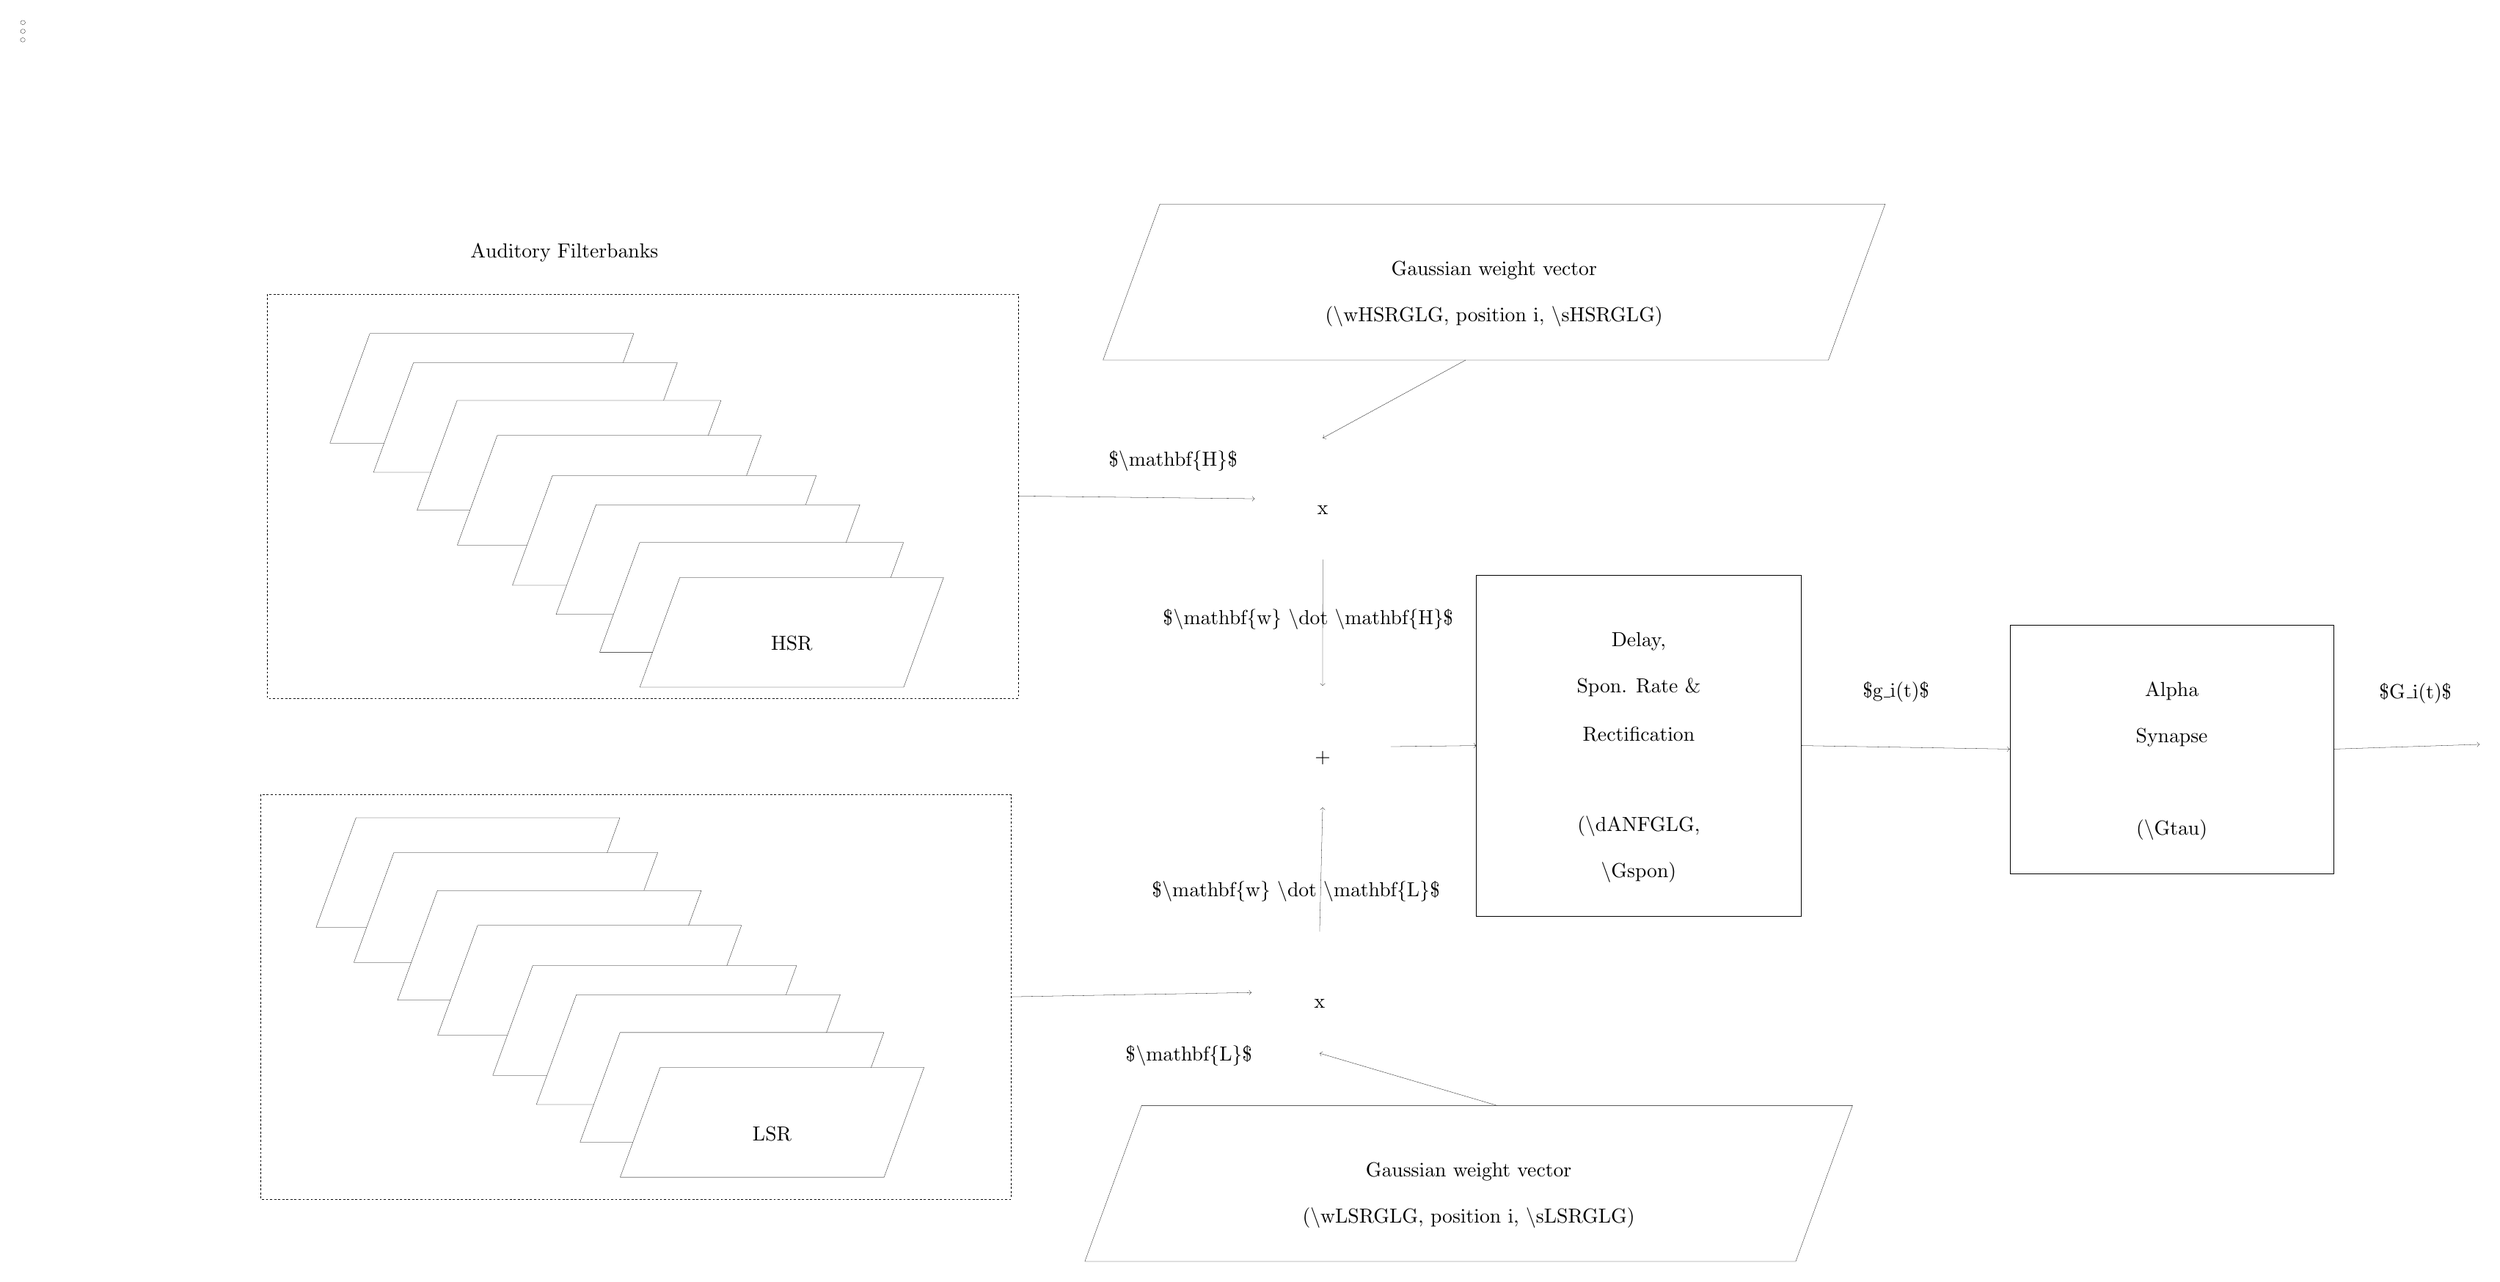
\begin{tikzpicture}
\pgftransformxscale{1.000000}
\pgftransformyscale{-1.000000}
\definecolor{dialinecolor}{rgb}{0.000000, 0.000000, 0.000000}
\pgfsetstrokecolor{dialinecolor}
\definecolor{dialinecolor}{rgb}{1.000000, 1.000000, 1.000000}
\pgfsetfillcolor{dialinecolor}
\definecolor{dialinecolor}{rgb}{1.000000, 1.000000, 1.000000}
\pgfsetfillcolor{dialinecolor}
\fill (5.050000\du,5.000000\du)--(5.050000\du,12.000000\du)--(18.050000\du,12.000000\du)--(18.050000\du,5.000000\du)--cycle;
\pgfsetlinewidth{0.100000\du}
\pgfsetdash{{1.000000\du}{1.000000\du}}{0\du}
\pgfsetdash{{1.000000\du}{1.000000\du}}{0\du}
\pgfsetmiterjoin
\definecolor{dialinecolor}{rgb}{0.000000, 0.000000, 0.000000}
\pgfsetstrokecolor{dialinecolor}
\draw (5.050000\du,5.000000\du)--(5.050000\du,12.000000\du)--(18.050000\du,12.000000\du)--(18.050000\du,5.000000\du)--cycle;
% setfont left to latex
\definecolor{dialinecolor}{rgb}{0.000000, 0.000000, 0.000000}
\pgfsetstrokecolor{dialinecolor}
\node at (11.550000\du,8.695000\du){};
\definecolor{dialinecolor}{rgb}{1.000000, 1.000000, 1.000000}
\pgfsetfillcolor{dialinecolor}
\fill (4.930000\du,13.671000\du)--(4.930000\du,20.671000\du)--(17.930000\du,20.671000\du)--(17.930000\du,13.671000\du)--cycle;
\pgfsetlinewidth{0.100000\du}
\pgfsetdash{{1.000000\du}{1.000000\du}}{0\du}
\pgfsetdash{{1.000000\du}{1.000000\du}}{0\du}
\pgfsetmiterjoin
\definecolor{dialinecolor}{rgb}{0.000000, 0.000000, 0.000000}
\pgfsetstrokecolor{dialinecolor}
\draw (4.930000\du,13.671000\du)--(4.930000\du,20.671000\du)--(17.930000\du,20.671000\du)--(17.930000\du,13.671000\du)--cycle;
% setfont left to latex
\definecolor{dialinecolor}{rgb}{0.000000, 0.000000, 0.000000}
\pgfsetstrokecolor{dialinecolor}
\node at (11.430000\du,17.366000\du){};
\pgfsetlinewidth{0.100000\du}
\pgfsetdash{}{0pt}
\pgfsetdash{}{0pt}
\pgfsetbuttcap
{
\definecolor{dialinecolor}{rgb}{0.000000, 0.000000, 0.000000}
\pgfsetfillcolor{dialinecolor}
% was here!!!
\pgfsetarrowsend{to}
\definecolor{dialinecolor}{rgb}{0.000000, 0.000000, 0.000000}
\pgfsetstrokecolor{dialinecolor}
\draw (18.050000\du,8.500000\du)--(22.145000\du,8.546680\du);
}
\definecolor{dialinecolor}{rgb}{1.000000, 1.000000, 1.000000}
\pgfsetfillcolor{dialinecolor}
\pgfpathellipse{\pgfpoint{23.321664\du}{12.839282\du}}{\pgfpoint{1.178364\du}{0\du}}{\pgfpoint{0\du}{1.051682\du}}
\pgfusepath{fill}
\pgfsetlinewidth{0.100000\du}
\pgfsetdash{}{0pt}
\pgfsetdash{}{0pt}
\pgfsetmiterjoin
\definecolor{dialinecolor}{rgb}{0.000000, 0.000000, 0.000000}
\pgfsetstrokecolor{dialinecolor}
\pgfpathellipse{\pgfpoint{23.321664\du}{12.839282\du}}{\pgfpoint{1.178364\du}{0\du}}{\pgfpoint{0\du}{1.051682\du}}
\pgfusepath{stroke}
% setfont left to latex
\definecolor{dialinecolor}{rgb}{0.000000, 0.000000, 0.000000}
\pgfsetstrokecolor{dialinecolor}
\node at (23.321664\du,13.034282\du){+};
\definecolor{dialinecolor}{rgb}{1.000000, 1.000000, 1.000000}
\pgfsetfillcolor{dialinecolor}
\fill (35.216400\du,10.731700\du)--(35.216400\du,15.031700\du)--(40.828900\du,15.031700\du)--(40.828900\du,10.731700\du)--cycle;
\pgfsetlinewidth{0.100000\du}
\pgfsetdash{}{0pt}
\pgfsetdash{}{0pt}
\pgfsetmiterjoin
\definecolor{dialinecolor}{rgb}{0.000000, 0.000000, 0.000000}
\pgfsetstrokecolor{dialinecolor}
\draw (35.216400\du,10.731700\du)--(35.216400\du,15.031700\du)--(40.828900\du,15.031700\du)--(40.828900\du,10.731700\du)--cycle;
% setfont left to latex
\definecolor{dialinecolor}{rgb}{0.000000, 0.000000, 0.000000}
\pgfsetstrokecolor{dialinecolor}
\node at (38.022650\du,11.876700\du){Alpha};
% setfont left to latex
\definecolor{dialinecolor}{rgb}{0.000000, 0.000000, 0.000000}
\pgfsetstrokecolor{dialinecolor}
\node at (38.022650\du,12.676700\du){Synapse};
% setfont left to latex
\definecolor{dialinecolor}{rgb}{0.000000, 0.000000, 0.000000}
\pgfsetstrokecolor{dialinecolor}
\node at (38.022650\du,13.476700\du){};
% setfont left to latex
\definecolor{dialinecolor}{rgb}{0.000000, 0.000000, 0.000000}
\pgfsetstrokecolor{dialinecolor}
\node at (38.022650\du,14.276700\du){(\ensuremath{\backslash}Gtau)};
\pgfsetlinewidth{0.100000\du}
\pgfsetdash{}{0pt}
\pgfsetdash{}{0pt}
\pgfsetbuttcap
{
\definecolor{dialinecolor}{rgb}{0.000000, 0.000000, 0.000000}
\pgfsetfillcolor{dialinecolor}
% was here!!!
\pgfsetarrowsend{to}
\definecolor{dialinecolor}{rgb}{0.000000, 0.000000, 0.000000}
\pgfsetstrokecolor{dialinecolor}
\draw (26.341200\du,19.053600\du)--(23.268900\du,18.148400\du);
}
\pgfsetlinewidth{0.100000\du}
\pgfsetdash{}{0pt}
\pgfsetdash{}{0pt}
\pgfsetbuttcap
{
\definecolor{dialinecolor}{rgb}{0.000000, 0.000000, 0.000000}
\pgfsetfillcolor{dialinecolor}
% was here!!!
\pgfsetarrowsend{to}
\definecolor{dialinecolor}{rgb}{0.000000, 0.000000, 0.000000}
\pgfsetstrokecolor{dialinecolor}
\draw (23.323400\du,9.598360\du)--(23.321600\du,11.787600\du);
}
% setfont left to latex
\definecolor{dialinecolor}{rgb}{0.000000, 0.000000, 0.000000}
\pgfsetstrokecolor{dialinecolor}
\node[anchor=west] at (8.450000\du,4.290980\du){Auditory Filterbanks};
\pgfsetlinewidth{0.100000\du}
\pgfsetdash{}{0pt}
\pgfsetdash{}{0pt}
\pgfsetbuttcap
{
\definecolor{dialinecolor}{rgb}{0.000000, 0.000000, 0.000000}
\pgfsetfillcolor{dialinecolor}
% was here!!!
\pgfsetarrowsend{to}
\definecolor{dialinecolor}{rgb}{0.000000, 0.000000, 0.000000}
\pgfsetstrokecolor{dialinecolor}
\draw (24.500000\du,12.839300\du)--(25.982500\du,12.821000\du);
}
\definecolor{dialinecolor}{rgb}{1.000000, 1.000000, 1.000000}
\pgfsetfillcolor{dialinecolor}
\fill (25.982500\du,9.871000\du)--(25.982500\du,15.771000\du)--(31.605000\du,15.771000\du)--(31.605000\du,9.871000\du)--cycle;
\pgfsetlinewidth{0.100000\du}
\pgfsetdash{}{0pt}
\pgfsetdash{}{0pt}
\pgfsetmiterjoin
\definecolor{dialinecolor}{rgb}{0.000000, 0.000000, 0.000000}
\pgfsetstrokecolor{dialinecolor}
\draw (25.982500\du,9.871000\du)--(25.982500\du,15.771000\du)--(31.605000\du,15.771000\du)--(31.605000\du,9.871000\du)--cycle;
% setfont left to latex
\definecolor{dialinecolor}{rgb}{0.000000, 0.000000, 0.000000}
\pgfsetstrokecolor{dialinecolor}
\node at (28.793750\du,11.016000\du){Delay, };
% setfont left to latex
\definecolor{dialinecolor}{rgb}{0.000000, 0.000000, 0.000000}
\pgfsetstrokecolor{dialinecolor}
\node at (28.793750\du,11.816000\du){Spon. Rate \&};
% setfont left to latex
\definecolor{dialinecolor}{rgb}{0.000000, 0.000000, 0.000000}
\pgfsetstrokecolor{dialinecolor}
\node at (28.793750\du,12.616000\du){Rectification};
% setfont left to latex
\definecolor{dialinecolor}{rgb}{0.000000, 0.000000, 0.000000}
\pgfsetstrokecolor{dialinecolor}
\node at (28.793750\du,13.416000\du){};
% setfont left to latex
\definecolor{dialinecolor}{rgb}{0.000000, 0.000000, 0.000000}
\pgfsetstrokecolor{dialinecolor}
\node at (28.793750\du,14.216000\du){(\ensuremath{\backslash}dANFGLG,};
% setfont left to latex
\definecolor{dialinecolor}{rgb}{0.000000, 0.000000, 0.000000}
\pgfsetstrokecolor{dialinecolor}
\node at (28.793750\du,15.016000\du){\ensuremath{\backslash}Gspon)};
\pgfsetlinewidth{0.100000\du}
\pgfsetdash{}{0pt}
\pgfsetdash{}{0pt}
\pgfsetbuttcap
{
\definecolor{dialinecolor}{rgb}{0.000000, 0.000000, 0.000000}
\pgfsetfillcolor{dialinecolor}
% was here!!!
\pgfsetarrowsend{to}
\definecolor{dialinecolor}{rgb}{0.000000, 0.000000, 0.000000}
\pgfsetstrokecolor{dialinecolor}
\draw (40.828900\du,12.881700\du)--(43.350000\du,12.800000\du);
}
\pgfsetlinewidth{0.100000\du}
\pgfsetdash{}{0pt}
\pgfsetdash{}{0pt}
\pgfsetbuttcap
{
\definecolor{dialinecolor}{rgb}{0.000000, 0.000000, 0.000000}
\pgfsetfillcolor{dialinecolor}
% was here!!!
\pgfsetarrowsend{to}
\definecolor{dialinecolor}{rgb}{0.000000, 0.000000, 0.000000}
\pgfsetstrokecolor{dialinecolor}
\draw (31.605000\du,12.821000\du)--(35.216400\du,12.881700\du);
}
\definecolor{dialinecolor}{rgb}{1.000000, 1.000000, 1.000000}
\pgfsetfillcolor{dialinecolor}
\fill (6.826543\du,5.685000\du)--(11.394558\du,5.685000\du)--(10.703015\du,7.585000\du)--(6.135000\du,7.585000\du)--cycle;
\pgfsetlinewidth{0.100000\du}
\pgfsetdash{}{0pt}
\pgfsetdash{}{0pt}
\pgfsetmiterjoin
\definecolor{dialinecolor}{rgb}{0.000000, 0.000000, 0.000000}
\pgfsetstrokecolor{dialinecolor}
\draw (6.826543\du,5.685000\du)--(11.394558\du,5.685000\du)--(10.703015\du,7.585000\du)--(6.135000\du,7.585000\du)--cycle;
% setfont left to latex
\definecolor{dialinecolor}{rgb}{0.000000, 0.000000, 0.000000}
\pgfsetstrokecolor{dialinecolor}
\node at (8.764779\du,6.830000\du){HSR};
\definecolor{dialinecolor}{rgb}{1.000000, 1.000000, 1.000000}
\pgfsetfillcolor{dialinecolor}
\fill (7.581543\du,6.190000\du)--(12.149558\du,6.190000\du)--(11.458015\du,8.090000\du)--(6.890000\du,8.090000\du)--cycle;
\pgfsetlinewidth{0.100000\du}
\pgfsetdash{}{0pt}
\pgfsetdash{}{0pt}
\pgfsetmiterjoin
\definecolor{dialinecolor}{rgb}{0.000000, 0.000000, 0.000000}
\pgfsetstrokecolor{dialinecolor}
\draw (7.581543\du,6.190000\du)--(12.149558\du,6.190000\du)--(11.458015\du,8.090000\du)--(6.890000\du,8.090000\du)--cycle;
% setfont left to latex
\definecolor{dialinecolor}{rgb}{0.000000, 0.000000, 0.000000}
\pgfsetstrokecolor{dialinecolor}
\node at (9.519779\du,7.335000\du){HSR};
\definecolor{dialinecolor}{rgb}{1.000000, 1.000000, 1.000000}
\pgfsetfillcolor{dialinecolor}
\fill (8.336543\du,6.845000\du)--(12.904558\du,6.845000\du)--(12.213015\du,8.745000\du)--(7.645000\du,8.745000\du)--cycle;
\pgfsetlinewidth{0.100000\du}
\pgfsetdash{}{0pt}
\pgfsetdash{}{0pt}
\pgfsetmiterjoin
\definecolor{dialinecolor}{rgb}{0.000000, 0.000000, 0.000000}
\pgfsetstrokecolor{dialinecolor}
\draw (8.336543\du,6.845000\du)--(12.904558\du,6.845000\du)--(12.213015\du,8.745000\du)--(7.645000\du,8.745000\du)--cycle;
% setfont left to latex
\definecolor{dialinecolor}{rgb}{0.000000, 0.000000, 0.000000}
\pgfsetstrokecolor{dialinecolor}
\node at (10.274779\du,7.990000\du){HSR};
\definecolor{dialinecolor}{rgb}{1.000000, 1.000000, 1.000000}
\pgfsetfillcolor{dialinecolor}
\fill (9.031983\du,7.450000\du)--(13.599998\du,7.450000\du)--(12.908455\du,9.350000\du)--(8.340440\du,9.350000\du)--cycle;
\pgfsetlinewidth{0.100000\du}
\pgfsetdash{}{0pt}
\pgfsetdash{}{0pt}
\pgfsetmiterjoin
\definecolor{dialinecolor}{rgb}{0.000000, 0.000000, 0.000000}
\pgfsetstrokecolor{dialinecolor}
\draw (9.031983\du,7.450000\du)--(13.599998\du,7.450000\du)--(12.908455\du,9.350000\du)--(8.340440\du,9.350000\du)--cycle;
% setfont left to latex
\definecolor{dialinecolor}{rgb}{0.000000, 0.000000, 0.000000}
\pgfsetstrokecolor{dialinecolor}
\node at (10.970219\du,8.595000\du){HSR};
\definecolor{dialinecolor}{rgb}{1.000000, 1.000000, 1.000000}
\pgfsetfillcolor{dialinecolor}
\fill (9.986543\du,8.145000\du)--(14.554558\du,8.145000\du)--(13.863015\du,10.045000\du)--(9.295000\du,10.045000\du)--cycle;
\pgfsetlinewidth{0.100000\du}
\pgfsetdash{}{0pt}
\pgfsetdash{}{0pt}
\pgfsetmiterjoin
\definecolor{dialinecolor}{rgb}{0.000000, 0.000000, 0.000000}
\pgfsetstrokecolor{dialinecolor}
\draw (9.986543\du,8.145000\du)--(14.554558\du,8.145000\du)--(13.863015\du,10.045000\du)--(9.295000\du,10.045000\du)--cycle;
% setfont left to latex
\definecolor{dialinecolor}{rgb}{0.000000, 0.000000, 0.000000}
\pgfsetstrokecolor{dialinecolor}
\node at (11.924779\du,9.290000\du){HSR};
\definecolor{dialinecolor}{rgb}{1.000000, 1.000000, 1.000000}
\pgfsetfillcolor{dialinecolor}
\fill (10.741543\du,8.650000\du)--(15.309558\du,8.650000\du)--(14.618015\du,10.550000\du)--(10.050000\du,10.550000\du)--cycle;
\pgfsetlinewidth{0.100000\du}
\pgfsetdash{}{0pt}
\pgfsetdash{}{0pt}
\pgfsetmiterjoin
\definecolor{dialinecolor}{rgb}{0.000000, 0.000000, 0.000000}
\pgfsetstrokecolor{dialinecolor}
\draw (10.741543\du,8.650000\du)--(15.309558\du,8.650000\du)--(14.618015\du,10.550000\du)--(10.050000\du,10.550000\du)--cycle;
% setfont left to latex
\definecolor{dialinecolor}{rgb}{0.000000, 0.000000, 0.000000}
\pgfsetstrokecolor{dialinecolor}
\node at (12.679779\du,9.795000\du){HSR};
\definecolor{dialinecolor}{rgb}{1.000000, 1.000000, 1.000000}
\pgfsetfillcolor{dialinecolor}
\fill (11.496543\du,9.305000\du)--(16.064558\du,9.305000\du)--(15.373015\du,11.205000\du)--(10.805000\du,11.205000\du)--cycle;
\pgfsetlinewidth{0.100000\du}
\pgfsetdash{}{0pt}
\pgfsetdash{}{0pt}
\pgfsetmiterjoin
\definecolor{dialinecolor}{rgb}{0.000000, 0.000000, 0.000000}
\pgfsetstrokecolor{dialinecolor}
\draw (11.496543\du,9.305000\du)--(16.064558\du,9.305000\du)--(15.373015\du,11.205000\du)--(10.805000\du,11.205000\du)--cycle;
% setfont left to latex
\definecolor{dialinecolor}{rgb}{0.000000, 0.000000, 0.000000}
\pgfsetstrokecolor{dialinecolor}
\node at (13.434779\du,10.450000\du){HSR};
\definecolor{dialinecolor}{rgb}{1.000000, 1.000000, 1.000000}
\pgfsetfillcolor{dialinecolor}
\fill (12.191943\du,9.910000\du)--(16.759958\du,9.910000\du)--(16.068415\du,11.810000\du)--(11.500400\du,11.810000\du)--cycle;
\pgfsetlinewidth{0.100000\du}
\pgfsetdash{}{0pt}
\pgfsetdash{}{0pt}
\pgfsetmiterjoin
\definecolor{dialinecolor}{rgb}{0.000000, 0.000000, 0.000000}
\pgfsetstrokecolor{dialinecolor}
\draw (12.191943\du,9.910000\du)--(16.759958\du,9.910000\du)--(16.068415\du,11.810000\du)--(11.500400\du,11.810000\du)--cycle;
% setfont left to latex
\definecolor{dialinecolor}{rgb}{0.000000, 0.000000, 0.000000}
\pgfsetstrokecolor{dialinecolor}
\node at (14.130179\du,11.055000\du){HSR};
\definecolor{dialinecolor}{rgb}{1.000000, 1.000000, 1.000000}
\pgfsetfillcolor{dialinecolor}
\fill (6.586543\du,14.070000\du)--(11.154558\du,14.070000\du)--(10.463015\du,15.970000\du)--(5.895000\du,15.970000\du)--cycle;
\pgfsetlinewidth{0.100000\du}
\pgfsetdash{}{0pt}
\pgfsetdash{}{0pt}
\pgfsetmiterjoin
\definecolor{dialinecolor}{rgb}{0.000000, 0.000000, 0.000000}
\pgfsetstrokecolor{dialinecolor}
\draw (6.586543\du,14.070000\du)--(11.154558\du,14.070000\du)--(10.463015\du,15.970000\du)--(5.895000\du,15.970000\du)--cycle;
% setfont left to latex
\definecolor{dialinecolor}{rgb}{0.000000, 0.000000, 0.000000}
\pgfsetstrokecolor{dialinecolor}
\node at (8.524779\du,15.215000\du){HSR};
\definecolor{dialinecolor}{rgb}{1.000000, 1.000000, 1.000000}
\pgfsetfillcolor{dialinecolor}
\fill (7.241543\du,14.675000\du)--(11.809558\du,14.675000\du)--(11.118015\du,16.575000\du)--(6.550000\du,16.575000\du)--cycle;
\pgfsetlinewidth{0.100000\du}
\pgfsetdash{}{0pt}
\pgfsetdash{}{0pt}
\pgfsetmiterjoin
\definecolor{dialinecolor}{rgb}{0.000000, 0.000000, 0.000000}
\pgfsetstrokecolor{dialinecolor}
\draw (7.241543\du,14.675000\du)--(11.809558\du,14.675000\du)--(11.118015\du,16.575000\du)--(6.550000\du,16.575000\du)--cycle;
% setfont left to latex
\definecolor{dialinecolor}{rgb}{0.000000, 0.000000, 0.000000}
\pgfsetstrokecolor{dialinecolor}
\node at (9.179779\du,15.820000\du){HSR};
\definecolor{dialinecolor}{rgb}{1.000000, 1.000000, 1.000000}
\pgfsetfillcolor{dialinecolor}
\fill (7.996543\du,15.330000\du)--(12.564558\du,15.330000\du)--(11.873015\du,17.230000\du)--(7.305000\du,17.230000\du)--cycle;
\pgfsetlinewidth{0.100000\du}
\pgfsetdash{}{0pt}
\pgfsetdash{}{0pt}
\pgfsetmiterjoin
\definecolor{dialinecolor}{rgb}{0.000000, 0.000000, 0.000000}
\pgfsetstrokecolor{dialinecolor}
\draw (7.996543\du,15.330000\du)--(12.564558\du,15.330000\du)--(11.873015\du,17.230000\du)--(7.305000\du,17.230000\du)--cycle;
% setfont left to latex
\definecolor{dialinecolor}{rgb}{0.000000, 0.000000, 0.000000}
\pgfsetstrokecolor{dialinecolor}
\node at (9.934779\du,16.475000\du){HSR};
\definecolor{dialinecolor}{rgb}{1.000000, 1.000000, 1.000000}
\pgfsetfillcolor{dialinecolor}
\fill (8.691983\du,15.935000\du)--(13.259998\du,15.935000\du)--(12.568455\du,17.835000\du)--(8.000440\du,17.835000\du)--cycle;
\pgfsetlinewidth{0.100000\du}
\pgfsetdash{}{0pt}
\pgfsetdash{}{0pt}
\pgfsetmiterjoin
\definecolor{dialinecolor}{rgb}{0.000000, 0.000000, 0.000000}
\pgfsetstrokecolor{dialinecolor}
\draw (8.691983\du,15.935000\du)--(13.259998\du,15.935000\du)--(12.568455\du,17.835000\du)--(8.000440\du,17.835000\du)--cycle;
% setfont left to latex
\definecolor{dialinecolor}{rgb}{0.000000, 0.000000, 0.000000}
\pgfsetstrokecolor{dialinecolor}
\node at (10.630219\du,17.080000\du){HSR};
\definecolor{dialinecolor}{rgb}{1.000000, 1.000000, 1.000000}
\pgfsetfillcolor{dialinecolor}
\fill (9.646543\du,16.630000\du)--(14.214558\du,16.630000\du)--(13.523015\du,18.530000\du)--(8.955000\du,18.530000\du)--cycle;
\pgfsetlinewidth{0.100000\du}
\pgfsetdash{}{0pt}
\pgfsetdash{}{0pt}
\pgfsetmiterjoin
\definecolor{dialinecolor}{rgb}{0.000000, 0.000000, 0.000000}
\pgfsetstrokecolor{dialinecolor}
\draw (9.646543\du,16.630000\du)--(14.214558\du,16.630000\du)--(13.523015\du,18.530000\du)--(8.955000\du,18.530000\du)--cycle;
% setfont left to latex
\definecolor{dialinecolor}{rgb}{0.000000, 0.000000, 0.000000}
\pgfsetstrokecolor{dialinecolor}
\node at (11.584779\du,17.775000\du){HSR};
\definecolor{dialinecolor}{rgb}{1.000000, 1.000000, 1.000000}
\pgfsetfillcolor{dialinecolor}
\fill (10.401543\du,17.135000\du)--(14.969558\du,17.135000\du)--(14.278015\du,19.035000\du)--(9.710000\du,19.035000\du)--cycle;
\pgfsetlinewidth{0.100000\du}
\pgfsetdash{}{0pt}
\pgfsetdash{}{0pt}
\pgfsetmiterjoin
\definecolor{dialinecolor}{rgb}{0.000000, 0.000000, 0.000000}
\pgfsetstrokecolor{dialinecolor}
\draw (10.401543\du,17.135000\du)--(14.969558\du,17.135000\du)--(14.278015\du,19.035000\du)--(9.710000\du,19.035000\du)--cycle;
% setfont left to latex
\definecolor{dialinecolor}{rgb}{0.000000, 0.000000, 0.000000}
\pgfsetstrokecolor{dialinecolor}
\node at (12.339779\du,18.280000\du){HSR};
\definecolor{dialinecolor}{rgb}{1.000000, 1.000000, 1.000000}
\pgfsetfillcolor{dialinecolor}
\fill (11.156543\du,17.790000\du)--(15.724558\du,17.790000\du)--(15.033015\du,19.690000\du)--(10.465000\du,19.690000\du)--cycle;
\pgfsetlinewidth{0.100000\du}
\pgfsetdash{}{0pt}
\pgfsetdash{}{0pt}
\pgfsetmiterjoin
\definecolor{dialinecolor}{rgb}{0.000000, 0.000000, 0.000000}
\pgfsetstrokecolor{dialinecolor}
\draw (11.156543\du,17.790000\du)--(15.724558\du,17.790000\du)--(15.033015\du,19.690000\du)--(10.465000\du,19.690000\du)--cycle;
% setfont left to latex
\definecolor{dialinecolor}{rgb}{0.000000, 0.000000, 0.000000}
\pgfsetstrokecolor{dialinecolor}
\node at (13.094779\du,18.935000\du){HSR};
\definecolor{dialinecolor}{rgb}{1.000000, 1.000000, 1.000000}
\pgfsetfillcolor{dialinecolor}
\fill (11.851943\du,18.395000\du)--(16.419958\du,18.395000\du)--(15.728415\du,20.295000\du)--(11.160400\du,20.295000\du)--cycle;
\pgfsetlinewidth{0.100000\du}
\pgfsetdash{}{0pt}
\pgfsetdash{}{0pt}
\pgfsetmiterjoin
\definecolor{dialinecolor}{rgb}{0.000000, 0.000000, 0.000000}
\pgfsetstrokecolor{dialinecolor}
\draw (11.851943\du,18.395000\du)--(16.419958\du,18.395000\du)--(15.728415\du,20.295000\du)--(11.160400\du,20.295000\du)--cycle;
% setfont left to latex
\definecolor{dialinecolor}{rgb}{0.000000, 0.000000, 0.000000}
\pgfsetstrokecolor{dialinecolor}
\node at (13.790179\du,19.540000\du){LSR};
% setfont left to latex
\definecolor{dialinecolor}{rgb}{0.000000, 0.000000, 0.000000}
\pgfsetstrokecolor{dialinecolor}
\node[anchor=west] at (32.550000\du,11.900000\du){\$g\_i(t)\$};
% setfont left to latex
\definecolor{dialinecolor}{rgb}{0.000000, 0.000000, 0.000000}
\pgfsetstrokecolor{dialinecolor}
\node[anchor=west] at (19.495000\du,7.890000\du){\$\ensuremath{\backslash}mathbf\{H\}\$};
\definecolor{dialinecolor}{rgb}{1.000000, 1.000000, 1.000000}
\pgfsetfillcolor{dialinecolor}
\pgfpathellipse{\pgfpoint{23.323364\du}{8.546682\du}}{\pgfpoint{1.178364\du}{0\du}}{\pgfpoint{0\du}{1.051682\du}}
\pgfusepath{fill}
\pgfsetlinewidth{0.100000\du}
\pgfsetdash{}{0pt}
\pgfsetdash{}{0pt}
\pgfsetmiterjoin
\definecolor{dialinecolor}{rgb}{0.000000, 0.000000, 0.000000}
\pgfsetstrokecolor{dialinecolor}
\pgfpathellipse{\pgfpoint{23.323364\du}{8.546682\du}}{\pgfpoint{1.178364\du}{0\du}}{\pgfpoint{0\du}{1.051682\du}}
\pgfusepath{stroke}
% setfont left to latex
\definecolor{dialinecolor}{rgb}{0.000000, 0.000000, 0.000000}
\pgfsetstrokecolor{dialinecolor}
\node at (23.323364\du,8.741682\du){x};
\pgfsetlinewidth{0.100000\du}
\pgfsetdash{}{0pt}
\pgfsetdash{}{0pt}
\pgfsetbuttcap
{
\definecolor{dialinecolor}{rgb}{0.000000, 0.000000, 0.000000}
\pgfsetfillcolor{dialinecolor}
% was here!!!
\pgfsetarrowsend{to}
\definecolor{dialinecolor}{rgb}{0.000000, 0.000000, 0.000000}
\pgfsetstrokecolor{dialinecolor}
\draw (17.930000\du,17.171000\du)--(22.090600\du,17.096700\du);
}
\pgfsetlinewidth{0.100000\du}
\pgfsetdash{}{0pt}
\pgfsetdash{}{0pt}
\pgfsetbuttcap
{
\definecolor{dialinecolor}{rgb}{0.000000, 0.000000, 0.000000}
\pgfsetfillcolor{dialinecolor}
% was here!!!
\pgfsetarrowsend{to}
\definecolor{dialinecolor}{rgb}{0.000000, 0.000000, 0.000000}
\pgfsetstrokecolor{dialinecolor}
\draw (23.268900\du,16.045000\du)--(23.321700\du,13.891000\du);
}
\definecolor{dialinecolor}{rgb}{1.000000, 1.000000, 1.000000}
\pgfsetfillcolor{dialinecolor}
\pgfpathellipse{\pgfpoint{23.268964\du}{17.096682\du}}{\pgfpoint{1.178364\du}{0\du}}{\pgfpoint{0\du}{1.051682\du}}
\pgfusepath{fill}
\pgfsetlinewidth{0.100000\du}
\pgfsetdash{}{0pt}
\pgfsetdash{}{0pt}
\pgfsetmiterjoin
\definecolor{dialinecolor}{rgb}{0.000000, 0.000000, 0.000000}
\pgfsetstrokecolor{dialinecolor}
\pgfpathellipse{\pgfpoint{23.268964\du}{17.096682\du}}{\pgfpoint{1.178364\du}{0\du}}{\pgfpoint{0\du}{1.051682\du}}
\pgfusepath{stroke}
% setfont left to latex
\definecolor{dialinecolor}{rgb}{0.000000, 0.000000, 0.000000}
\pgfsetstrokecolor{dialinecolor}
\node at (23.268964\du,17.291682\du){x};
\definecolor{dialinecolor}{rgb}{1.000000, 1.000000, 1.000000}
\pgfsetfillcolor{dialinecolor}
\fill (20.502420\du,3.445000\du)--(33.059772\du,3.445000\du)--(32.077052\du,6.145000\du)--(19.519700\du,6.145000\du)--cycle;
\pgfsetlinewidth{0.100000\du}
\pgfsetdash{}{0pt}
\pgfsetdash{}{0pt}
\pgfsetmiterjoin
\definecolor{dialinecolor}{rgb}{0.000000, 0.000000, 0.000000}
\pgfsetstrokecolor{dialinecolor}
\draw (20.502420\du,3.445000\du)--(33.059772\du,3.445000\du)--(32.077052\du,6.145000\du)--(19.519700\du,6.145000\du)--cycle;
% setfont left to latex
\definecolor{dialinecolor}{rgb}{0.000000, 0.000000, 0.000000}
\pgfsetstrokecolor{dialinecolor}
\node at (26.289736\du,4.590000\du){Gaussian weight vector};
% setfont left to latex
\definecolor{dialinecolor}{rgb}{0.000000, 0.000000, 0.000000}
\pgfsetstrokecolor{dialinecolor}
\node at (26.289736\du,5.390000\du){(\ensuremath{\backslash}wHSRGLG, position i, \ensuremath{\backslash}sHSRGLG)};
% setfont left to latex
\definecolor{dialinecolor}{rgb}{0.000000, 0.000000, 0.000000}
\pgfsetstrokecolor{dialinecolor}
\node[anchor=west] at (19.795000\du,18.190000\du){\$\ensuremath{\backslash}mathbf\{L\}\$};
% setfont left to latex
\definecolor{dialinecolor}{rgb}{0.000000, 0.000000, 0.000000}
\pgfsetstrokecolor{dialinecolor}
\node[anchor=west] at (20.250000\du,15.350000\du){\$\ensuremath{\backslash}mathbf\{w\} \ensuremath{\backslash}dot \ensuremath{\backslash}mathbf\{L\}\$};
% setfont left to latex
\definecolor{dialinecolor}{rgb}{0.000000, 0.000000, 0.000000}
\pgfsetstrokecolor{dialinecolor}
\node[anchor=west] at (20.445000\du,10.640000\du){\$\ensuremath{\backslash}mathbf\{w\} \ensuremath{\backslash}dot \ensuremath{\backslash}mathbf\{H\}\$};
\pgfsetlinewidth{0.100000\du}
\pgfsetdash{}{0pt}
\pgfsetdash{}{0pt}
\pgfsetbuttcap
{
\definecolor{dialinecolor}{rgb}{0.000000, 0.000000, 0.000000}
\pgfsetfillcolor{dialinecolor}
% was here!!!
\pgfsetarrowsend{to}
\definecolor{dialinecolor}{rgb}{0.000000, 0.000000, 0.000000}
\pgfsetstrokecolor{dialinecolor}
\draw (25.798400\du,6.145000\du)--(23.323400\du,7.495000\du);
}
\definecolor{dialinecolor}{rgb}{1.000000, 1.000000, 1.000000}
\pgfsetfillcolor{dialinecolor}
\fill (20.187520\du,19.053600\du)--(32.494872\du,19.053600\du)--(31.512152\du,21.753600\du)--(19.204800\du,21.753600\du)--cycle;
\pgfsetlinewidth{0.100000\du}
\pgfsetdash{}{0pt}
\pgfsetdash{}{0pt}
\pgfsetmiterjoin
\definecolor{dialinecolor}{rgb}{0.000000, 0.000000, 0.000000}
\pgfsetstrokecolor{dialinecolor}
\draw (20.187520\du,19.053600\du)--(32.494872\du,19.053600\du)--(31.512152\du,21.753600\du)--(19.204800\du,21.753600\du)--cycle;
% setfont left to latex
\definecolor{dialinecolor}{rgb}{0.000000, 0.000000, 0.000000}
\pgfsetstrokecolor{dialinecolor}
\node at (25.849836\du,20.198600\du){Gaussian weight vector};
% setfont left to latex
\definecolor{dialinecolor}{rgb}{0.000000, 0.000000, 0.000000}
\pgfsetstrokecolor{dialinecolor}
\node at (25.849836\du,20.998600\du){(\ensuremath{\backslash}wLSRGLG, position i, \ensuremath{\backslash}sLSRGLG)};
% setfont left to latex
\definecolor{dialinecolor}{rgb}{0.000000, 0.000000, 0.000000}
\pgfsetstrokecolor{dialinecolor}
\node[anchor=west] at (41.495000\du,11.915000\du){\$G\_i(t)\$};
\end{tikzpicture}
}\\
\caption[Golgi cell model diagram]{The Golgi instantaneous-rate profile was generated using a weighted sum ANF profiles and a alpha function smoothing filter to mimic dendritic and synaptic filtering.
The Gaussian spread of connections is independent for HSR and LSR auditory filters, with the mean equal to CF channel of unit.
The final stage sets the spontaneous rate by addition at t=0, changes any negative values to zero, and includes an additional delay of 2.5~ms, which is 0.7~ms greater than the core VCN units as shown by \citet{GhoshalKim:1997}.}
% across frequency channels is Gaussian, and $\mathbf{w}$ is
% the weighted sum of HSR and LSR instantaneous-rate vectors,
% $\alpha$ is the synaptic and dendritic smoothing function.
  \label{fig:GolgiDiagram}
 \end{figure}
%\smallskip{}

The weight vectors, $\mathbf{w}_{HSR}$ and $\mathbf{w}_{LSR}$, span the network's channels with size $N_{\rm channel}$, with a normal curve centred on the position in the channel and variance \sANFGLG\@.
Instantaneous-rate profiles of the \AN~have size $N_{\rm channel}$ and length determined by the stimulus ($N_{\rm stim}=$stimulus duration / sampling rate).
The intermediate step in the Golgi cell model, $r(\cdot)$, corrects the output rate for the desired spontaneous activity, \Gspon, and performs rectification on the signal to avoid negative rate values.
The final step involves convolution with the alpha function, $\alpha(t)$, as the synapto-dendritic filtering mechanism in the Golgi cell.
The alpha filter length was 10 times the time constant, \Gtau, and its area under the function was normalised to 1.
A more detailed explanation of the NEURON implementation of the Golgi cell model is in the section Appendix~\ref{sec:ch3:appendix}.

%\smallskip{}
% Eq.~\ref{eq:alpha_Golgi},
% In Chapter~\ref{sec:GAChapter}, the Golgi cell model was implemented as a
% single-compartment conductance neuron. Due to the unavailability of sufficient
% data regarding \emph{in vivo} Golgi cell responses, the decision was made to
% simulate the Golgi cell model as a Poisson neuron.  The instantaneous-rate
% profile of Golgi cells use inputs from the auditory model's instantaneous rate
% outputs, and a number of steps were taken to investigate the Golgi cell model.

%\smallskip{}
% Due to its replication of granule cells in the model, weight for \LSR~(\wLSRGLG) and \HSR~(\wHSRGLG) are determined for all synapses, number \nLSRDS~and \nHSRDS, delay \dANFGLG~added to smoothing function to ensure conductance
% and dendritic filtering are included.

% \subsubsection{Key design factors}
% \yellownote{TODO: expand para, include fig ref} Choosing neural model: \HH-type
% or Poisson - Problem of monotonic excitation at low levels - Spread of \ANF~to
% \GCD~ARE broader than core \VCN- are we spoiling the broth too early?
% \includegraphics[width=0.6\textwidth,angle=-90]{GolgiRateLevelActualFit}\\
% \caption{Optimisation Results for Golgi Model using Rate Level data from
% \label{Ch3:fig:GolgiFit}}
%\includegraphics[width=0.8\textwidth]{GolgiRateLevel}\\
%\caption{Optimisation Results for Golgi Model using Rate Level data from
% \label{Ch3:fig:GolgiRL}}
%\includegraphics[width=0.8\textwidth]{golgi_RateLevel_opt}\\
%\caption{Optimisation Results for Golgi Model using Rate Level data from
% \label{Ch3:fig:GolgiRL}}
%\includegraphics[width=0.8\textwidth,angle=-90]{GolgiRateLevel2}\\
%\caption{Optimisation Results for Golgi Model using Rate Level data from
% \label{Ch3:fig:GolgiRL}}

%%% Local Variables:
%%% mode: latex
%%% mode: tex-fold
%%% mode: visual-line
%%% TeX-master: "SimpleResponses"
%%% TeX-PDF-mode: nil
%%% End:
